% answers.tex —— 1977 年·山东B卷 · 参考答案与详细解析片段
% 由 tools/generate_projects.py 依来源总账自 1977/1977_数学真题_山东B_试题.md + 1977/1977_数学真题_山东B_解析正文.md + 1977/1977_数学真题_山东B_答案要点.md 生成，勿手改（改源 MD 后重跑）


\begin{gktip}
固定源 PDF 为题面与解答连续排印的扫描材料（书籍页码 57—63）。下文逐题独立推导，并与源卷所附「解：」对照复算，两者一致。原卷第一大题的 6 个小题在本库中为第 1—6 题，原第二至六大题依次为第 7—11 题（见试题卷首题号说明）；卷末参考题两道的解析接在第 11 题之后。
\end{gktip}

\begin{answer}
\gksolhead{1}{}

\textbf{题目}：

$\sqrt{(-a)^2}=?$

\Needspace{4\baselineskip}
\textbf{解析}

\Needspace{5\baselineskip}
$(\,-a\,)^2=a^2$，对其开方取算术根，结果由 $a$ 的符号分情况：

\nopagebreak[4]
\[
\sqrt{(-a)^2}=|a|=
\begin{cases}
a & (a\ge 0),\\
-a & (a<0).
\end{cases}
\]

与源卷解答一致。

\gkanswer{答案：当 $a\ge 0$ 时为 $a$，当 $a<0$ 时为 $-a$（即 $\sqrt{(-a)^2}=|a|$）。}

\end{answer}
\begin{answer}
\gksolhead{2}{}

\textbf{题目}：

$\log_{\frac{1}{2}}\left[\left(1-\cos^2\dfrac{\pi}{6}\right)\operatorname{ctg}^{-2}\dfrac{\pi}{4}\right]=?$

\Needspace{4\baselineskip}
\textbf{解析}

\Needspace{5\baselineskip}
由 $\cos^2\dfrac{\pi}{6}=\dfrac34$，得 $1-\cos^2\dfrac{\pi}{6}=\dfrac14=\sin^2\dfrac{\pi}{6}$；又 $\operatorname{ctg}\dfrac{\pi}{4}=1$，其负二次幂

\nopagebreak[4]
\[
\operatorname{ctg}^{-2}\frac{\pi}{4}
=\frac{1}{\operatorname{ctg}^2\frac{\pi}{4}}
=\operatorname{tg}^2\frac{\pi}{4}=1.
\]

\Needspace{5\baselineskip}
于是

\nopagebreak[4]
\[
\begin{aligned}
\text{\text{原式}}
&=\log_{\frac12}\left[\left(1-\cos^2\frac{\pi}{6}\right)\operatorname{ctg}^{-2}\frac{\pi}{4}\right]\\
&=\log_{\frac12}\left(\frac14\cdot 1\right)=2.
\end{aligned}
\]

与源卷解答（原式等于 $\log_{\frac12}\bigl[(1-\tfrac34)\cdot1\bigr]=2$）一致。

\gkanswer{答案：$2$。}

\end{answer}
\begin{answer}
\gksolhead{3}{}

\textbf{题目}：

写出下列函数的定义域：

（1） $y=\dfrac{\sqrt{|x-3|}}{x-2}$；

（2） $y=\lg(x+3)$.

\Needspace{4\baselineskip}
\textbf{解析}

\gksubpart{（1）}

\Needspace{5\baselineskip}
分子根式 $\sqrt{|x-3|}$ 的被开方数 $|x-3|\ge 0$ 对一切实数成立，根式总有意义；只有分母有限制：

\nopagebreak[4]
\[
x-2\ne 0,
\qquad\text{\text{即}}\ x\ne 2.
\]

\gksubpart{（2）}

\Needspace{5\baselineskip}
对数的真数必须为正：

\nopagebreak[4]
\[
x+3>0
\qquad\text{\text{即}}\ x>-3.
\]

\gkanswer{答案（1）：$x\ne 2$。}

\gkanswer{答案（2）：$x>-3$。}

\end{answer}
\begin{answer}
\gksolhead{4}{}

\textbf{题目}：

写出过 $(0,\ 1)$ 和 $(2,\ 3)$ 两点的直线方程.

\Needspace{4\baselineskip}
\textbf{解析}

\Needspace{5\baselineskip}
由直线方程的两点式，

\nopagebreak[4]
\[
\frac{y-1}{3-1}=\frac{x-0}{2-0},
\]

\Needspace{5\baselineskip}
即 $y-1=x$，化简得

\nopagebreak[4]
\[
x-y+1=0.
\]

\gkanswer{答案：$x-y+1=0$。}

\end{answer}
\begin{answer}
\gksolhead{5}{}

\textbf{题目}：

写出双曲线 $\dfrac{x^2}{16}-\dfrac{y^2}{9}=1$ 的渐近线方程.

\Needspace{4\baselineskip}
\textbf{解析}

\Needspace{5\baselineskip}
与双曲线 $\dfrac{x^2}{a^2}-\dfrac{y^2}{b^2}=1$ 对应，$a=4$、$b=3$，故渐近线方程为

\nopagebreak[4]
\[
\frac{x}{4}\pm\frac{y}{3}=0.
\]

\gkanswer{答案：$\dfrac{x}{4}\pm\dfrac{y}{3}=0$。}

\end{answer}
\begin{answer}
\gksolhead{6}{}

\textbf{题目}：

如图所示的二视图是什么几何体？
\nopagebreak[4]
\begin{center}% 1977 年山东B卷第 6 题：正四棱锥的二视图（按源卷第 2 页布局）
% 上：正面图（三角形，垂直点划中心线）；下：俯视图（正方形加两条对角线，十字中心线）
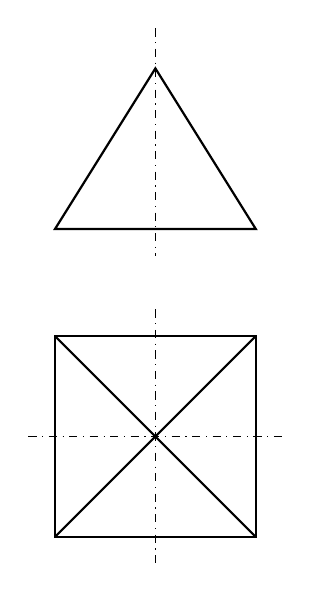
\begin{tikzpicture}[scale=0.85]
  % ---- 正面图：三角形 ----
  \coordinate (apex) at (0,2.4);
  \coordinate (bl) at (-1.5,0);
  \coordinate (br) at (1.5,0);
  \draw[thick] (bl)--(apex)--(br)--cycle;
  % 正面图垂直中心线（点划线，超出图形）
  \draw[dash dot] (0,3.0)--(0,-0.4);
  % ---- 俯视图：正方形 + 对角线 ----
  \coordinate (s1) at (-1.5,-1.6);
  \coordinate (s2) at (1.5,-1.6);
  \coordinate (s3) at (1.5,-4.6);
  \coordinate (s4) at (-1.5,-4.6);
  \draw[thick] (s1)--(s2)--(s3)--(s4)--cycle;
  \draw[thick] (s1)--(s3);
  \draw[thick] (s2)--(s4);
  % 俯视图十字中心线（点划线，超出图形）
  \draw[dash dot] (0,-1.2)--(0,-5.0);
  \draw[dash dot] (-1.9,-3.1)--(1.9,-3.1);
\end{tikzpicture}
\end{center}
\nopagebreak[4]
\Needspace{4\baselineskip}
\textbf{解析}

二视图由两部分组成。正面图是一个三角形，说明该几何体是锥体；俯视图是带两条对角线的正方形，说明底面是正方形，且锥顶在底面的投影位于对角线交点（即底面中心）。两者合成，该几何体是正四棱锥。
\nopagebreak[4]
\begin{center}% 1977 年山东B卷第 6 题：正四棱锥的二视图（按源卷第 2 页布局）
% 上：正面图（三角形，垂直点划中心线）；下：俯视图（正方形加两条对角线，十字中心线）
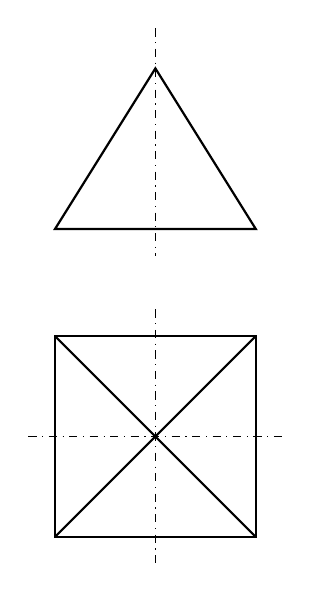
\begin{tikzpicture}[scale=0.85]
  % ---- 正面图：三角形 ----
  \coordinate (apex) at (0,2.4);
  \coordinate (bl) at (-1.5,0);
  \coordinate (br) at (1.5,0);
  \draw[thick] (bl)--(apex)--(br)--cycle;
  % 正面图垂直中心线（点划线，超出图形）
  \draw[dash dot] (0,3.0)--(0,-0.4);
  % ---- 俯视图：正方形 + 对角线 ----
  \coordinate (s1) at (-1.5,-1.6);
  \coordinate (s2) at (1.5,-1.6);
  \coordinate (s3) at (1.5,-4.6);
  \coordinate (s4) at (-1.5,-4.6);
  \draw[thick] (s1)--(s2)--(s3)--(s4)--cycle;
  \draw[thick] (s1)--(s3);
  \draw[thick] (s2)--(s4);
  % 俯视图十字中心线（点划线，超出图形）
  \draw[dash dot] (0,-1.2)--(0,-5.0);
  \draw[dash dot] (-1.9,-3.1)--(1.9,-3.1);
\end{tikzpicture}
\end{center}
\nopagebreak[4]
\gkanswer{答案：正四棱锥。}

\end{answer}
\begin{answer}
\gksolhead{7}{}

\textbf{题目}：

$\square ABCD$ 的二邻边之比为 $1:2$，$M$ 为大边 $AB$ 的中点，连接 $MD$、$MC$，求证：$\angle DMC=\dfrac{\pi}{2}$.
\nopagebreak[4]
\begin{center}% 1977 年山东B卷第 7 题：平行四边形 ABCD，M 为大边 AB 的中点，连接 MD、MC（按源卷第 3 页布局）
% D 左上、C 右上、A 左下、M 在 AB 中点、B 右下
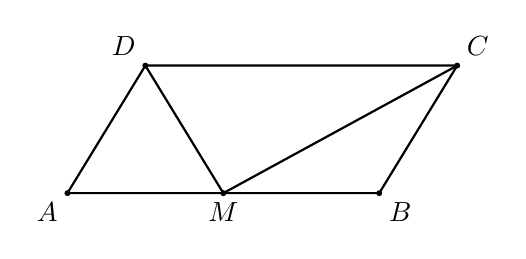
\begin{tikzpicture}[scale=0.9]
  \coordinate (A) at (0,0);
  \coordinate (M) at (2.2,0);
  \coordinate (B) at (4.4,0);
  \coordinate (D) at (1.1,1.8);
  \coordinate (C) at (5.5,1.8);
  \draw[thick] (A)--(B)--(C)--(D)--cycle;
  \draw[thick] (D)--(M);
  \draw[thick] (M)--(C);
  \fill (A) circle (1.2pt) node[below left] {$A$};
  \fill (M) circle (1.2pt) node[below] {$M$};
  \fill (B) circle (1.2pt) node[below right] {$B$};
  \fill (D) circle (1.2pt) node[above left] {$D$};
  \fill (C) circle (1.2pt) node[above right] {$C$};
\end{tikzpicture}
\end{center}
\nopagebreak[4]
\Needspace{4\baselineskip}
\textbf{解析}

\Needspace{5\baselineskip}
由二邻边之比 $AB:AD=1:2$ 知 $AB=2\,AD$。$M$ 为大边 $AB$ 的中点，故

\nopagebreak[4]
\[
AM=\frac12\,AB=AD.
\]

\Needspace{5\baselineskip}
在 $\triangle MAD$ 中，由 $AM=AD$ 得

\nopagebreak[4]
\[
\angle ADM=\angle AMD.
\]

\Needspace{5\baselineskip}
又 $AB\parallel DC$，$AM$、$MD$ 为截线两侧，内错角

\nopagebreak[4]
\[
\angle AMD=\angle MDC,
\]

\Needspace{5\baselineskip}
从而 $\angle ADM=\angle MDC$，即

\nopagebreak[4]
\[
\angle MDC=\frac12\,\angle ADC.
\]

\Needspace{5\baselineskip}
再由 $BC=AD=MB$（$BC$ 等于对边 $AD$，又等于半边 $MB$），在 $\triangle MBC$ 中同理得

\nopagebreak[4]
\[
\angle MCD=\frac12\,\angle BCD.
\]

\Needspace{5\baselineskip}
两式相加，并利用平行四边形同旁内角 $\angle ADC+\angle BCD=\pi$：

\nopagebreak[4]
\[
\begin{aligned}
\angle MDC+\angle MCD
&=\frac12\,(\angle ADC+\angle BCD)\\
&=\frac12\times\pi=\frac{\pi}{2}.
\end{aligned}
\]

\Needspace{5\baselineskip}
在 $\triangle MDC$ 中，

\nopagebreak[4]
\[
\angle DMC=\pi-(\angle MDC+\angle MCD)=\frac{\pi}{2}.
\]
\nopagebreak[4]
\begin{center}% 1977 年山东B卷第 7 题：平行四边形 ABCD，M 为大边 AB 的中点，连接 MD、MC（按源卷第 3 页布局）
% D 左上、C 右上、A 左下、M 在 AB 中点、B 右下
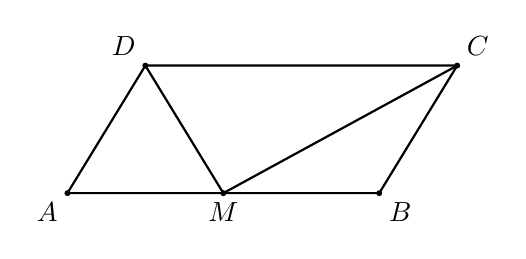
\begin{tikzpicture}[scale=0.9]
  \coordinate (A) at (0,0);
  \coordinate (M) at (2.2,0);
  \coordinate (B) at (4.4,0);
  \coordinate (D) at (1.1,1.8);
  \coordinate (C) at (5.5,1.8);
  \draw[thick] (A)--(B)--(C)--(D)--cycle;
  \draw[thick] (D)--(M);
  \draw[thick] (M)--(C);
  \fill (A) circle (1.2pt) node[below left] {$A$};
  \fill (M) circle (1.2pt) node[below] {$M$};
  \fill (B) circle (1.2pt) node[below right] {$B$};
  \fill (D) circle (1.2pt) node[above left] {$D$};
  \fill (C) circle (1.2pt) node[above right] {$C$};
\end{tikzpicture}
\end{center}
\nopagebreak[4]
\gkanswer{答案：见解析版}

\end{answer}
\begin{answer}
\gksolhead{8}{}

\Needspace{5\baselineskip}
\textbf{题目}：

\nopagebreak[4]
\[
\frac{\sin\alpha}{2}\,x^2+x+\frac{1}{2\cos\alpha}=0
\qquad\left(0<\alpha<\frac{\pi}{2}\right)
\]

为关于 $x$ 的二次方程。当 $\alpha$ 为何值时，方程有两个不相等的实数根？它的根是什么？

\Needspace{4\baselineskip}
\textbf{解析}

\Needspace{5\baselineskip}
二次方程 $ax^2+bx+c=0$ 的系数为

\nopagebreak[4]
\[
a=\frac{\sin\alpha}{2},
\qquad b=1,
\qquad c=\frac{1}{2\cos\alpha}.
\]

\Needspace{5\baselineskip}
判别式

\nopagebreak[4]
\[
\begin{aligned}
b^2-4ac
&=1-4\cdot\frac{\sin\alpha}{2}\cdot\frac{1}{2\cos\alpha}\\
&=1-\frac{\sin\alpha}{\cos\alpha}=1-\operatorname{tg}\alpha.
\end{aligned}
\]

\Needspace{5\baselineskip}
方程有两个不相等实数根的条件是

\nopagebreak[4]
\[
1-\operatorname{tg}\alpha>0,
\qquad\text{\text{即}}\ \operatorname{tg}\alpha<1.
\]

\Needspace{5\baselineskip}
结合 $0<\alpha<\dfrac{\pi}{2}$，得

\nopagebreak[4]
\[
0<\alpha<\frac{\pi}{4}.
\]

\Needspace{5\baselineskip}
由求根公式，

\nopagebreak[4]
\[
x=\frac{-1\pm\sqrt{1-\operatorname{tg}\alpha}}{2\cdot\frac{\sin\alpha}{2}}
=\frac{-1\pm\sqrt{1-\operatorname{tg}\alpha}}{\sin\alpha}.
\]

与源卷解答的根式一致。

\gkanswer{答案：当 $0<\alpha<\dfrac{\pi}{4}$ 时，方程有两个不相等的实数根，根为 $x=\dfrac{-1\pm\sqrt{1-\operatorname{tg}\alpha}}{\sin\alpha}$。}

\end{answer}
\begin{answer}
\gksolhead{9}{}

\textbf{题目}：

试比较等底等高的正四棱锥和正圆锥的侧面积，看哪个的侧面积较小.

\Needspace{4\baselineskip}
\textbf{解析}

设正四棱锥和圆锥的底面积均为 $S$，高均为 $h$。

\Needspace{5\baselineskip}
正四棱锥的底面边长为 $\sqrt{S}$，斜高为

\nopagebreak[4]
\[
\sqrt{\left(\frac{\sqrt{S}}{2}\right)^2+h^2}
=\sqrt{\frac{S}{4}+h^2}.
\]

\Needspace{5\baselineskip}
侧面积为

\nopagebreak[4]
\[
\begin{aligned}
S_{\text{\text{正四棱锥侧}}}
&=4\cdot\frac12\cdot\sqrt{S}\cdot\sqrt{\frac{S}{4}+h^2}\\
&=\sqrt{S^2+4Sh^2}.
\end{aligned}
\]

\Needspace{5\baselineskip}
圆锥的底面半径 $r=\sqrt{\dfrac{S}{\pi}}$，母线

\nopagebreak[4]
\[
l=\sqrt{\left(\sqrt{\frac{S}{\pi}}\right)^2+h^2}
=\sqrt{\frac{S}{\pi}+h^2}.
\]

\Needspace{5\baselineskip}
侧面积为

\nopagebreak[4]
\[
\begin{aligned}
S_{\text{\text{圆锥侧}}}
&=\pi\cdot\sqrt{\frac{S}{\pi}}\cdot\sqrt{\frac{S}{\pi}+h^2}\\
&=\sqrt{S^2+\pi Sh^2}.
\end{aligned}
\]

\Needspace{5\baselineskip}
由 $\pi<4$ 得 $S^2+\pi Sh^2<S^2+4Sh^2$，所以

\nopagebreak[4]
\[
S_{\text{\text{圆锥侧}}}<S_{\text{\text{正四棱锥侧}}},
\]

即等底等高时圆锥的侧面积较小。

\gkanswer{答案：圆锥的侧面积较小：$S_{\text{\text{圆锥侧}}}<S_{\text{\text{正四棱锥侧}}}$。}

\end{answer}
\begin{answer}
\gksolhead{10}{}

\textbf{题目}：

一只船以 $v$ 海里/小时的速度向正北航行，在 $A$ 处望见灯塔在船的北 $\alpha$ 度东，继续航行 $t$ 小时后，在 $B$ 处望见 $S$ 在船的北 $\beta$ 度东，求第二次望见灯塔 $S$ 时船和灯塔的距离 $BS$.
\nopagebreak[4]
\begin{center}% 1977 年山东B卷第 10 题：船 A→B 向正北航行，灯塔 S 的方位角 α、β（按源卷第 5 页布局）
% A、B 在同一南北线上，S 在东北方向；β 标在 B 处，α 标在 A 处；右侧画北南西东方向标
\begin{tikzpicture}[scale=0.9,>=stealth]
  % 航线（南北线，虚线）
  \draw[dashed] (0,-0.5)--(0,4.9);
  \coordinate (A) at (0,0);
  \coordinate (B) at (0,3.2);
  \coordinate (S) at (1.9,4.3);
  \draw[thick] (A)--(S);
  \draw[thick] (B)--(S);
  \fill (S) circle (1.6pt);
  \node[above right] at (S) {$S$};
  \node[below left] at (A) {$A$};
  \node[left] at (B) {$B$};
  % A 处角 α（正北线与 AS 之间）
  \draw (0,0.75) arc[start angle=90,end angle=66,radius=0.75];
  \node at (0.30,0.92) {$\alpha$};
  % B 处角 β（正北线与 BS 之间）
  \draw (0,4.15) arc[start angle=90,end angle=30,radius=0.95];
  \node at (0.42,4.28) {$\beta$};
  % 方向标：北南西东
  \begin{scope}[shift={(2.9,1.5)}]
    \draw[->] (0,-0.9)--(0,0.9) node[above] {$\text{北}$};
    \node[below] at (0,-0.9) {$\text{南}$};
    \draw (-0.9,0)--(0.9,0);
    \draw[->] (0,0)--(0.9,0);
    \node[left] at (-0.9,0) {$\text{西}$};
    \node[right] at (0.9,0) {$\text{东}$};
  \end{scope}
\end{tikzpicture}
\end{center}
\nopagebreak[4]
\Needspace{4\baselineskip}
\textbf{解析}

\Needspace{5\baselineskip}
船沿正北方向航行，$A$、$B$ 在同一南北线上，$AB=vt$。在 $A$ 处，$AS$ 与正北方向的夹角为 $\alpha$，即 $\angle BAS=\alpha$；在 $B$ 处，$BS$ 与正北方向夹角为 $\beta$，而 $BA$ 指向正南，故

\nopagebreak[4]
\[
\angle ABS=\pi-\beta.
\]

\Needspace{5\baselineskip}
三角形内角和给出

\nopagebreak[4]
\[
\angle ASB=\pi-\alpha-(\pi-\beta)=\beta-\alpha.
\]

\Needspace{5\baselineskip}
由正弦定理，

\nopagebreak[4]
\[
\frac{BS}{\sin\alpha}=\frac{vt}{\sin(\beta-\alpha)},
\]

\Needspace{5\baselineskip}
所以

\nopagebreak[4]
\[
BS=\frac{vt\sin\alpha}{\sin(\beta-\alpha)}.
\]
\nopagebreak[4]
\begin{center}% 1977 年山东B卷第 10 题：船 A→B 向正北航行，灯塔 S 的方位角 α、β（按源卷第 5 页布局）
% A、B 在同一南北线上，S 在东北方向；β 标在 B 处，α 标在 A 处；右侧画北南西东方向标
\begin{tikzpicture}[scale=0.9,>=stealth]
  % 航线（南北线，虚线）
  \draw[dashed] (0,-0.5)--(0,4.9);
  \coordinate (A) at (0,0);
  \coordinate (B) at (0,3.2);
  \coordinate (S) at (1.9,4.3);
  \draw[thick] (A)--(S);
  \draw[thick] (B)--(S);
  \fill (S) circle (1.6pt);
  \node[above right] at (S) {$S$};
  \node[below left] at (A) {$A$};
  \node[left] at (B) {$B$};
  % A 处角 α（正北线与 AS 之间）
  \draw (0,0.75) arc[start angle=90,end angle=66,radius=0.75];
  \node at (0.30,0.92) {$\alpha$};
  % B 处角 β（正北线与 BS 之间）
  \draw (0,4.15) arc[start angle=90,end angle=30,radius=0.95];
  \node at (0.42,4.28) {$\beta$};
  % 方向标：北南西东
  \begin{scope}[shift={(2.9,1.5)}]
    \draw[->] (0,-0.9)--(0,0.9) node[above] {$\text{北}$};
    \node[below] at (0,-0.9) {$\text{南}$};
    \draw (-0.9,0)--(0.9,0);
    \draw[->] (0,0)--(0.9,0);
    \node[left] at (-0.9,0) {$\text{西}$};
    \node[right] at (0.9,0) {$\text{东}$};
  \end{scope}
\end{tikzpicture}
\end{center}
\nopagebreak[4]
\gkanswer{答案：$BS=\dfrac{vt\sin\alpha}{\sin(\beta-\alpha)}$。}

\end{answer}
\begin{answer}
\gksolhead{11}{}

\textbf{题目}：

某隧道的横断面如图所示，已知隧道横断面的周长为 $23$ 米，试根据图所示尺寸，求当 $x$ 和 $y$ 为何值时，隧道的横断面的面积最大？最大面积是多少？（取 $\pi\approx 3$）（图尺寸单位：米）
\nopagebreak[4]
\begin{center}% 1977 年山东B卷第 11 题：隧道横断面（按源卷第 5 页布局）
% 上为半圆（半径 x，拱顶），下为矩形（高 y）；底部中央有宽 2x-1、高 0.5 的凸台阶，
% 台阶下基线画虚线；底部两段各标 0.5，台阶竖高标 0.5
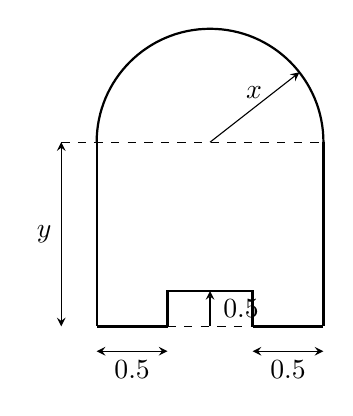
\begin{tikzpicture}[scale=0.9,>=stealth]
  % 半圆拱（圆心在拱弦线中点）
  \coordinate (L) at (-1.6,0);
  \coordinate (R) at (1.6,0);
  \draw[thick] (-1.6,0) arc[start angle=180,end angle=0,radius=1.6];
  % 拱弦线（虚线）
  \draw[dashed] (-2.1,0)--(1.6,0);
  % 半径 x 标注（箭头指向弧）
  \draw[->] (0,0)--(38:1.6);
  \node[above] at (0.62,0.48) {$x$};
  % 两侧竖墙
  \draw[thick] (-1.6,0)--(-1.6,-2.6);
  \draw[thick] (1.6,0)--(1.6,-2.6);
  % 底部：0.5 — 台阶（宽2x-1、高0.5）— 0.5
  \draw[thick] (-1.6,-2.6)--(-0.6,-2.6);
  \draw[thick] (-0.6,-2.6)--(-0.6,-2.1)--(0.6,-2.1)--(0.6,-2.6);
  \draw[thick] (0.6,-2.6)--(1.6,-2.6);
  % 台阶下基线（虚线）
  \draw[dashed] (-0.6,-2.6)--(0.6,-2.6);
  % 左侧高度 y 标注
  \draw[<->] (-2.1,0)--(-2.1,-2.6);
  \node[left] at (-2.1,-1.3) {$y$};
  % 底部左 0.5
  \draw[<->] (-1.6,-2.95)--(-0.6,-2.95);
  \node[below] at (-1.1,-2.95) {$0.5$};
  % 底部右 0.5
  \draw[<->] (0.6,-2.95)--(1.6,-2.95);
  \node[below] at (1.1,-2.95) {$0.5$};
  % 台阶高 0.5
  \draw[->] (0,-2.6)--(0,-2.1);
  \node[right] at (0.05,-2.35) {$0.5$};
\end{tikzpicture}
\end{center}
\nopagebreak[4]
\begin{gktip}
\textbf{参考题}
\end{gktip}

\Needspace{5\baselineskip}
\textbf{参考题 1．} 求极限：

\nopagebreak[4]
\[
\lim_{x\to0}\frac{\ln(1+x)}{x}.
\]

\textbf{参考题 2．} 用定积分求抛物线 $y^2=4x$ 与 $x^2=4y$ 所围成的曲边形面积.
\nopagebreak[4]
\begin{center}% 1977 年山东B卷参考题 2：抛物线 y²=4x 与 x²=4y 所围曲边形（按源卷第 6 页布局）
% 坐标轴标 X、Y，两抛物线按源卷记号标 X²=4Y（上）与 Y²=4X（右下），交点 (0,0) 与 (4,4)
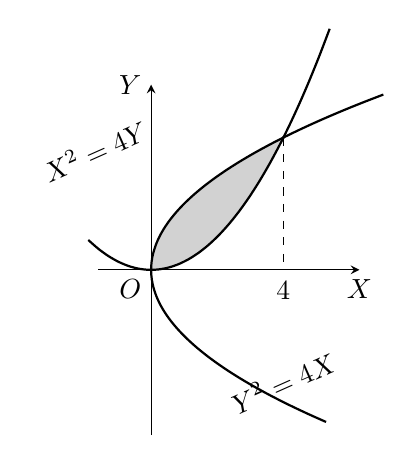
\begin{tikzpicture}[scale=0.42,>=stealth]
  % 坐标轴
  \draw[->] (-1.6,0)--(6.3,0) node[below] {$X$};
  \draw[->] (0,-5.0)--(0,5.6) node[left] {$Y$};
  \node[below left] at (0,0) {$O$};
  % 阴影区域：0≤x≤4 上 2√x 与 x²/4 之间
  \fill[gray!35]
    (0,0) plot[domain=0:4,smooth] (\x,{2*sqrt(\x)})
    -- plot[domain=4:0,smooth] (\x,{\x*\x/4}) -- cycle;
  % 抛物线 y²=4x（右开口，含左下延伸段）
  \draw[thick,domain=-4.6:5.3,smooth,samples=40] plot ({\x*\x/4},{\x});
  % 抛物线 x²=4y（上开口）
  \draw[thick,domain=-1.9:5.4,smooth] plot (\x,{\x*\x/4});
  % 交点 (4,4) 与虚线垂线
  \fill (4,4) circle (1.5pt);
  \draw[dashed] (4,4)--(4,0);
  \node[below] at (4,-0.05) {$4$};
  % 曲线标签（按源卷位置）
  \node[rotate=24] at (-1.7,3.6) {$X^2=4Y$};
  \node[rotate=24] at (4.0,-3.4) {$Y^2=4X$};
\end{tikzpicture}
\end{center}
\nopagebreak[4]
\Needspace{4\baselineskip}
\textbf{解析}

横断面由上半圆、矩形组成，底部中央有一个宽 $2x-1$、高 $0.5$ 米的凸台阶。周长由半圆弧（$\pi\approx3$，取 $3x$）、两侧竖边 $2y$、底部两段合计 $2x$ 与台阶两竖边 $0.5\times2$ 组成：
\nopagebreak[4]
\begin{center}% 1977 年山东B卷第 11 题：隧道横断面（按源卷第 5 页布局）
% 上为半圆（半径 x，拱顶），下为矩形（高 y）；底部中央有宽 2x-1、高 0.5 的凸台阶，
% 台阶下基线画虚线；底部两段各标 0.5，台阶竖高标 0.5
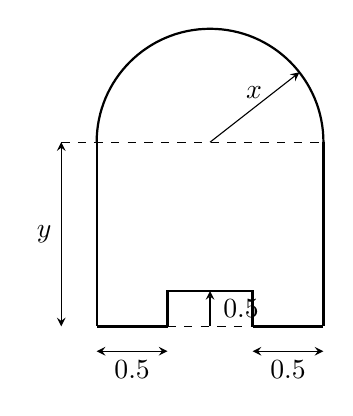
\begin{tikzpicture}[scale=0.9,>=stealth]
  % 半圆拱（圆心在拱弦线中点）
  \coordinate (L) at (-1.6,0);
  \coordinate (R) at (1.6,0);
  \draw[thick] (-1.6,0) arc[start angle=180,end angle=0,radius=1.6];
  % 拱弦线（虚线）
  \draw[dashed] (-2.1,0)--(1.6,0);
  % 半径 x 标注（箭头指向弧）
  \draw[->] (0,0)--(38:1.6);
  \node[above] at (0.62,0.48) {$x$};
  % 两侧竖墙
  \draw[thick] (-1.6,0)--(-1.6,-2.6);
  \draw[thick] (1.6,0)--(1.6,-2.6);
  % 底部：0.5 — 台阶（宽2x-1、高0.5）— 0.5
  \draw[thick] (-1.6,-2.6)--(-0.6,-2.6);
  \draw[thick] (-0.6,-2.6)--(-0.6,-2.1)--(0.6,-2.1)--(0.6,-2.6);
  \draw[thick] (0.6,-2.6)--(1.6,-2.6);
  % 台阶下基线（虚线）
  \draw[dashed] (-0.6,-2.6)--(0.6,-2.6);
  % 左侧高度 y 标注
  \draw[<->] (-2.1,0)--(-2.1,-2.6);
  \node[left] at (-2.1,-1.3) {$y$};
  % 底部左 0.5
  \draw[<->] (-1.6,-2.95)--(-0.6,-2.95);
  \node[below] at (-1.1,-2.95) {$0.5$};
  % 底部右 0.5
  \draw[<->] (0.6,-2.95)--(1.6,-2.95);
  \node[below] at (1.1,-2.95) {$0.5$};
  % 台阶高 0.5
  \draw[->] (0,-2.6)--(0,-2.1);
  \node[right] at (0.05,-2.35) {$0.5$};
\end{tikzpicture}
\end{center}
\nopagebreak[4]
\nopagebreak[4]
\[
3x+2y+2x+0.5\times2=23,
\]

\Needspace{5\baselineskip}
解得

\nopagebreak[4]
\[
y=(23-3x-0.5\times2-2x)\times\frac12=11-2.5x.
\]

\Needspace{5\baselineskip}
设横断面面积为 $S$，等于半圆面积 $\dfrac{3x^2}{2}$ 加矩形面积 $2xy$，再扣除台阶占用的 $(2x-1)\times0.5$：

\nopagebreak[4]
\[
\begin{aligned}
S&\approx\frac{3x^2}{2}+2x\,(11-2.5x)-(2x-1)\times0.5\\
&=-3.5x^2+21x+0.5.
\end{aligned}
\]

\Needspace{5\baselineskip}
由 $-3.5<0$，抛物线开口向下，在顶点处取最大值：

\nopagebreak[4]
\[
x=-\frac{21}{2\times(-3.5)}=3,
\]

\Needspace{5\baselineskip}
此时

\nopagebreak[4]
\[
\mathrm{S}_{\max}=\frac{4\times(-3.5)\times0.5-21^2}{4\times(-3.5)}=32\ \text{（\text{米}}^2\text{）}.
\]

当 $x=3$ 时，$y=11-2.5\times3=3.5$（米）。即半圆半径 $x$ 为 $3$ 米、$y$ 为 $3.5$ 米时横断面面积最大，最大面积为 $32$ 平方米。

\textbf{参考题 1}

\Needspace{5\baselineskip}
由洛必达法则（分子分母分别求导），

\nopagebreak[4]
\[
\lim_{x\to0}\frac{\ln(1+x)}{x}
=\lim_{x\to0}\frac{[\ln(1+x)]'}{x'}
=\lim_{x\to0}\frac{1}{1+x}=1.
\]

\textbf{参考题 2}

\Needspace{5\baselineskip}
解方程组

\nopagebreak[4]
\[
\begin{cases}
y^2=4x,\\
x^2=4y
\end{cases}
\]

得两交点的横坐标 $x=0$ 与 $x=4$。在 $0\le x\le4$ 上，上边界为 $y=2\sqrt{x}$（来自 $y^2=4x$），下边界为 $y=\dfrac{x^2}{4}$，故
\nopagebreak[4]
\begin{center}% 1977 年山东B卷参考题 2：抛物线 y²=4x 与 x²=4y 所围曲边形（按源卷第 6 页布局）
% 坐标轴标 X、Y，两抛物线按源卷记号标 X²=4Y（上）与 Y²=4X（右下），交点 (0,0) 与 (4,4)
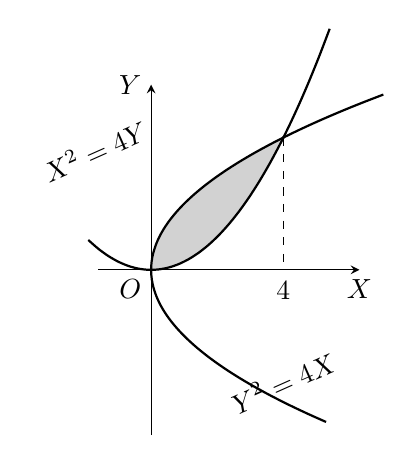
\begin{tikzpicture}[scale=0.42,>=stealth]
  % 坐标轴
  \draw[->] (-1.6,0)--(6.3,0) node[below] {$X$};
  \draw[->] (0,-5.0)--(0,5.6) node[left] {$Y$};
  \node[below left] at (0,0) {$O$};
  % 阴影区域：0≤x≤4 上 2√x 与 x²/4 之间
  \fill[gray!35]
    (0,0) plot[domain=0:4,smooth] (\x,{2*sqrt(\x)})
    -- plot[domain=4:0,smooth] (\x,{\x*\x/4}) -- cycle;
  % 抛物线 y²=4x（右开口，含左下延伸段）
  \draw[thick,domain=-4.6:5.3,smooth,samples=40] plot ({\x*\x/4},{\x});
  % 抛物线 x²=4y（上开口）
  \draw[thick,domain=-1.9:5.4,smooth] plot (\x,{\x*\x/4});
  % 交点 (4,4) 与虚线垂线
  \fill (4,4) circle (1.5pt);
  \draw[dashed] (4,4)--(4,0);
  \node[below] at (4,-0.05) {$4$};
  % 曲线标签（按源卷位置）
  \node[rotate=24] at (-1.7,3.6) {$X^2=4Y$};
  \node[rotate=24] at (4.0,-3.4) {$Y^2=4X$};
\end{tikzpicture}
\end{center}
\nopagebreak[4]
\nopagebreak[4]
\[
\begin{aligned}
S&=\int_0^4 2\sqrt{x}\,dx-\int_0^4\frac14x^2\,dx\\
&=2\cdot\frac23\,x^{\frac32}\,\bigg|_0^4-\frac14\cdot\frac13\,x^3\,\bigg|_0^4\\
&=\frac{32}{3}-\frac{16}{3}=\frac{16}{3}.
\end{aligned}
\]

\gkanswer{答案：当 $x=3$ 米、$y=3.5$ 米时，隧道横断面面积最大，最大面积为 $32$ 平方米。}

\end{answer}